%
% $RCSfile$
%
% Copyright (c) 2002-2006. Christian Heller. All rights reserved.
%
% Permission is granted to copy, distribute and/or modify this document
% under the terms of the GNU Free Documentation License, Version 1.1 or
% any later version published by the Free Software Foundation; with no
% Invariant Sections, with no Front-Cover Texts and with no Back-Cover
% Texts. A copy of the license is included in the section entitled
% "GNU Free Documentation License".
%
% http://www.cybop.net
% - Cybernetics Oriented Programming -
%
% http://www.resmedicinae.org
% - Information in Medicine -
%
% Version: $Revision$ $Date$ $Author$
% Authors: Christian Heller <christian.heller@tuxtax.de>
%

\subsubsection{Logic manipulates State}
\label{logic_manipulates_state_heading}

According to the observations made in the work described in this article, there
are two kinds of knowledge: \emph{States} and \emph{Logic}. While the former
may be placed in a spatial dimension, the latter is processed as sequence over
time. Often, logic is labelled \emph{dynamic} behaviour -- but only the
\emph{execution} of a rule of logic is dynamic, \emph{not} the rule itself
(\emph{static}).

Rules of logic translate input- into output states. What characterises a system
is how it applies logic knowledge to translate state knowledge \cite{heller2002}.
Yet how to imagine a knowledge model consisting of state- as well as logic
parts? Following an example. The famous \emph{Model View Controller} (MVC)
pattern was extended by the \emph{Hierarchical MVC} (HMVC) pattern towards a
hierarchy of \emph{MVC Triads} \cite{cai}. The omnipresence of hierarchies in
the MVC was demonstrated in \cite{hellerbohl}.

\begin{figure}[ht]
    \begin{center}
        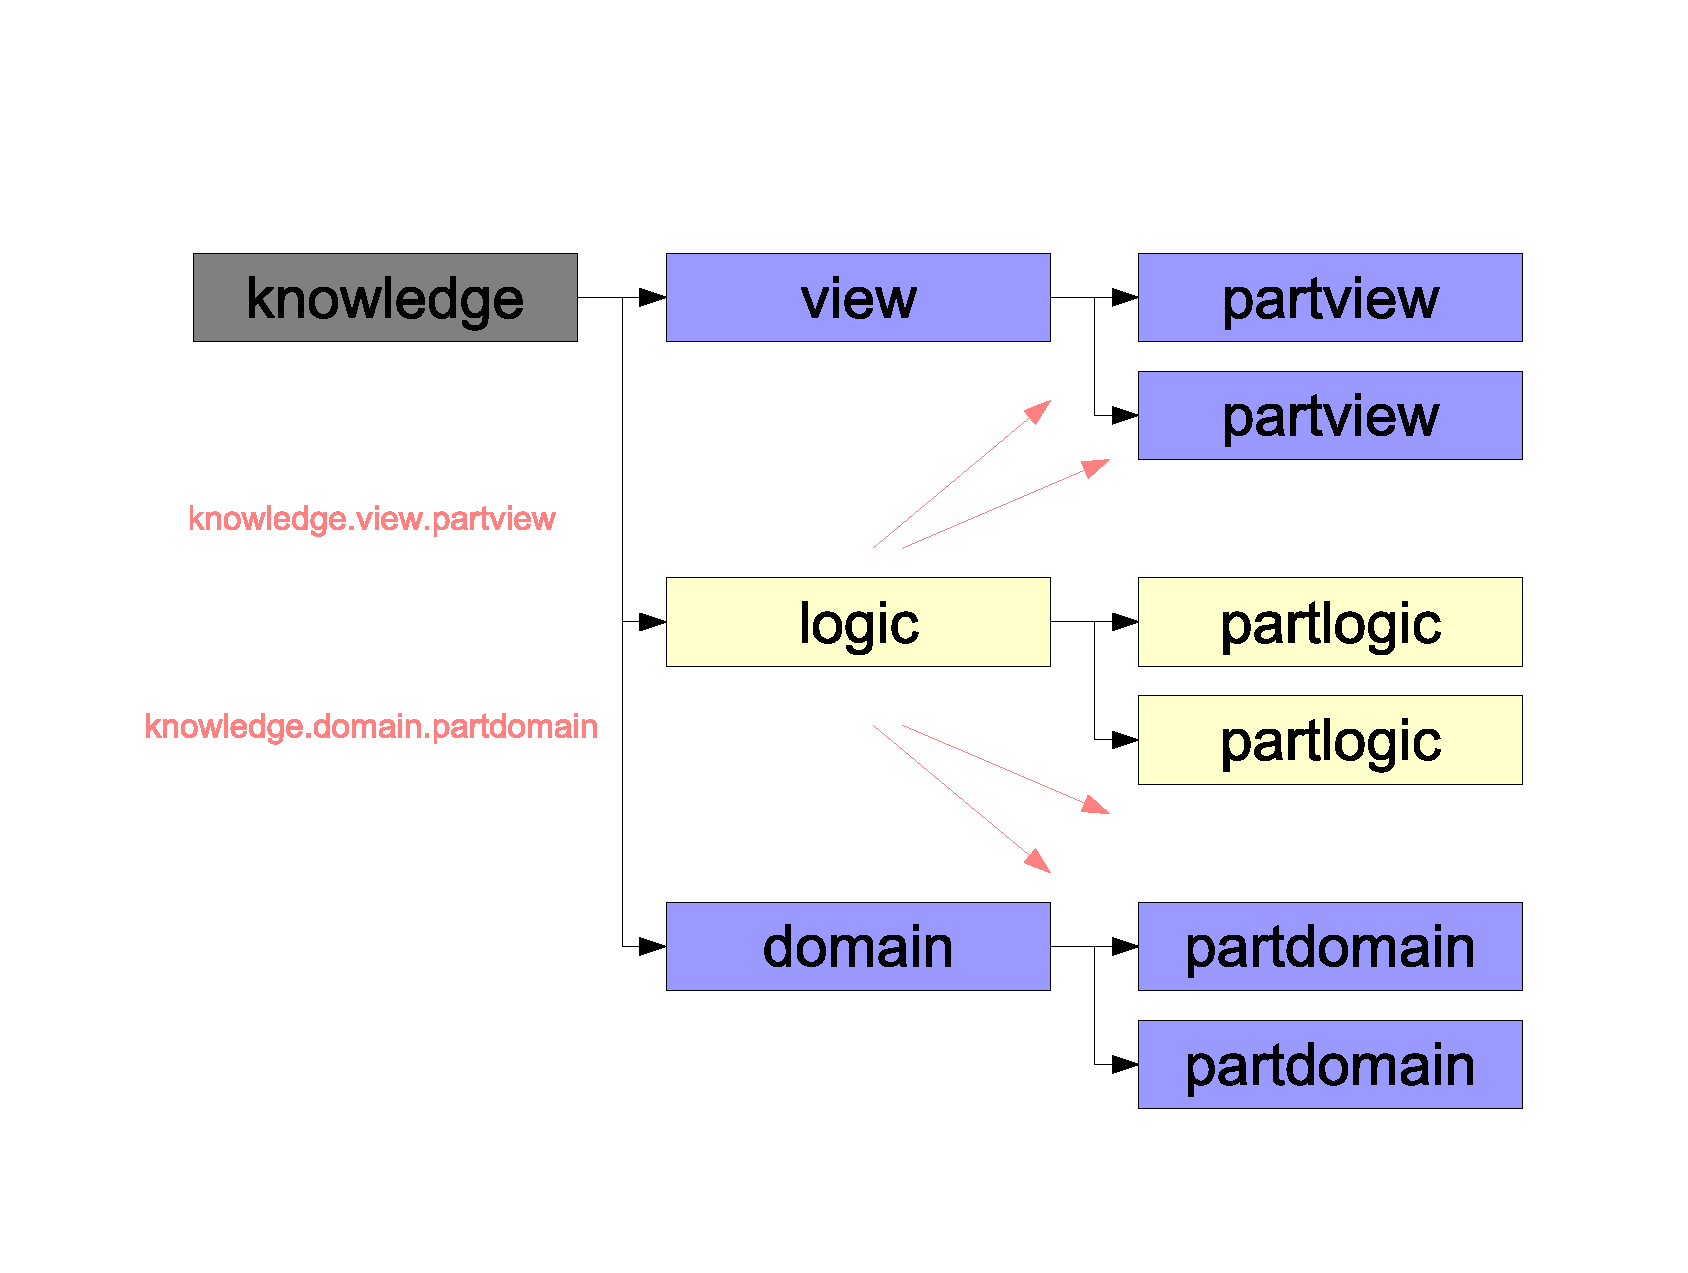
\includegraphics[scale=0.2]{vector/mvctree.eps}
        \caption{Logic manipulating States}
        \label{mvctree_figure}
    \end{center}
\end{figure}

Figure \ref{mvctree_figure} shows the three parts: \emph{Domain} (Model),
\emph{View} and \emph{Logic} (Controller) of an (adapted) MVC pattern as
independent branches of one common knowledge tree, as existent at system
runtime in memory. Each of them represents a concept on its own. The logic
model, however, is allowed to access and change the view- and domain model; it
is able to link different knowledge models. But view- and domain model,
representing states, are not allowed to manipulate logic. In other words: The
dependencies between logic- and state models are \emph{unidirectional}.

An innovation is that logic knowledge gets manipulatable. A logic model
(algorithm) cannot only access and change state-, but also logic models, even
itself! Because models modified in that manner can be made persistent in form
of CYBOL knowledge templates (section \ref{cybol_heading}), and be reloaded the
next time an application starts, this may be seen as a kind of
\emph{Meta Programming}, which \cite{wikipedia} defines as: \textit{the writing
of programs that write or manipulate other programs (or themselves) as their
data.}

The clear separation of states and logic into discrete models avoids unwanted
dependencies as caused by the bundling of attributes and methods in OOP. All
that would be needed to make a CYBOP system work with new state models, is the
corresponding translation logic. Translators \cite{hellerkunze} simplify
architectures and unify communication.
